\documentclass[]{article}
\usepackage{graphicx}
\usepackage{float}
\usepackage{amsmath}
\usepackage{verbatimbox}
\usepackage{textcomp}
\usepackage{fullpage}

\usepackage{listings}
\usepackage{color}
\usepackage[usenames,dvipsnames]{xcolor}
\definecolor{dkgreen}{rgb}{0,0.6,0}
\definecolor{gray}{rgb}{0.5,0.5,0.5}
\definecolor{mauve}{rgb}{0.58,0,0.82}

\lstset{frame=tb,
  language=C,
  aboveskip=3mm,
  belowskip=3mm,
  showstringspaces=false,
  columns=flexible,
  basicstyle={\small\ttfamily},
  numbers=left,
  numberstyle=\tiny\color{gray},
  keywordstyle=\color{blue},
  commentstyle=\color{dkgreen},
  stringstyle=\color{mauve},
  breaklines=true,
  breakatwhitespace=true,
  tabsize=3,
  otherkeywords={llu\_mi128i, arr\_m128i}
}

\bibliographystyle{plain}
%opening
\title{VNTR proposal}
\author{Elizabeth (Beth) Becker}

\begin{document}

\maketitle
\section{Overview of VNTRs}

For my final project, I will analyze data related to variable number tandem repeats (VNTRs). VNTRs are short sequences found in DNA that repeat. The number of times they repeat, or the copy number, vary from person to person. Irregular copy numbers can sometimes cause or be indicative of certain diseases. VNTRs are also used commonly in forensic and paternity testing. 

\section{Data Collection}
I am currently working in Dr. Gary Benson's lab, and was provided data about 148 individuals. For each individual, I have information on what VNTRs were found and what the copy numbers are. (Because humans have two of each chromosome, they could have different copy numbers on different chromosomes). Each person has a reference ID and each VNTR also has an ID. The copy number data was provided as a string with the format \#/\#, where each \# is the number of copies compared the reference number. 

 In these people, 3827 VNTRs have been detected. However, a lot of data is missing. On average 42.02\% of people have information about a given VNTR. For some, only one person has information, for others, all 148 individuals have data. There is also a list of VNTRs that were found, but are likely flawed. After filtering those out, there are 2598 VNTRs left. I wanted understand better what my data looked like so I made a histogram, shown below. If I had data about every VNTR for every person, this graph would have one bar at 148 that was 2598 tall. As you can see, this is not the case. I have a lot of VNTRs where only 1 or 2 people have data on it. There are very few VNTRs where I have data for all 148 people. 

\begin{figure}[H]
	\centering
    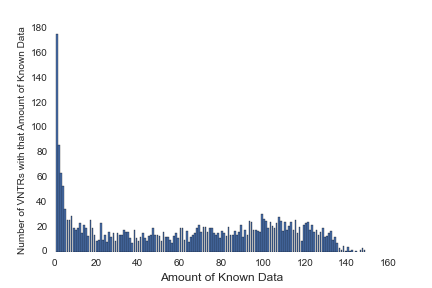
\includegraphics[width=7cm,height=7cm,keepaspectratio]{histogram.png}
    \caption{Graph helps give an idea of how much data is missing.}
\end{figure}
 The range of the copy numbers are from -72 (72 less than reference)to 7 (7 more than the reference). 
 
I was also provided with general information about known VNTRs. This is a list of 226,782 different VNTRs, which chromosome they are on, their location on that chromosome, the reference copy number, and the base sequence (which repeats).  In the reference information, the lowest copy number is 1.752809 and the highest is 629.322571.  

All the genomes from these individuals came from the 1000 Genomes project. From their website, I was able to download additional data. I have information on where the individuals are from (their population), their sex, whether they are known to have a disease, and their relationships between each other (some are families, with mother, father, and child). I thought I was going to have to webscrape for this information, but I found a way to download it instead. I was able to determine how many people are from what populations:
\begin{center}
  \begin{tabular}{| c| c | c |}
      \hline
      abbreviation   & location & Number of Genomes \\ \hline
      ACB   & African Caribbean & 6 \\ \hline
      CEU   & Utah residents & 1 \\ \hline
      FIN   & Finnish & 11 \\ \hline
      GBR   & British & 18 \\ \hline
      IBS   & Spanish Iberian & 25 \\ \hline
      KHV   & Kinh Vietnamese & 12 \\ \hline
      PEL   & Peruvian & 16 \\ \hline
      PUR   & Puerto Rico & 32 \\ \hline
   \end{tabular}
 \end{center}
 
 
\section{Data Processing Plans}
As mentioned before, I removed all the flawed data from the set of VNTRs and genomes that I had.
For each individual there are two numbers for a given VNTR, one for each chromosome. I will be treating the data as categorical data. A genotype is a specific genetic feature. Having a specific copy number of a VNTR is one version (or allele) of a genotype. For each allele, I will make a category. For instance, for the VNTR with reference number 182168820, I will have \textcolor{red}{1}182168820, with an extra 1 copy, \textcolor{red}{0}182168820 with 0 extra copies, \textcolor{red}{-1}182168820, with one fewer copy than reference. For each population, and also individual, I will count the number of times each allele occurred. I will divide by the number of detected alleles for that person or population. If there is no data for a specific allele, the relative number will be 0. This is a valid way for processing unknown data because certain VNTRs are fundamentally harder to process. 

I will be treating this data as categorical data because the processes that cause VNTRs to increase or decrease their copy number are fairly rare. 

\section{Hypothesizes}
I plan to hierarchically cluster all the individuals. Individuals within populations should be more similar than those outside the population. Also, populations that are geographically closer, or share histories should be more genetically similar than others.

I will also hierarchically cluster all the populations. I should see a similar result the individual clustering, and hopefully the results will agree with each other.  

Additionally, I plan to see if I can make a predictor that could determine an individual's population based on their VNTR information for each population where I have more than 10 members. 

I also want to see if their is a linear correlation between the number of VNTRs found on a chromosome and the size of the chromosome.

I also want to see if men or women have more VNTRs. (I expect there to be no significant difference, except for VNTRs found on the X or Y chromosomes.)

I will also do a regression to see if the copy number of a VNTR could be modeled linearly or logarithmically with the length of the base sequence. 

Unfortunately, there was inadequate data on whether any of the individuals had diseases, so I will not be able to investigate that part. Also, there were no complete families included in the data set, so I will not be able to analyze that.  
\end{document}